\chapter{Clystyru k-modd}\label{cha:literature}
\section{Cefndir}\label{sec:axelrodoriginal}
Mae clystyru k-modd yn ffordd o ddysgu heb oruchwyliaeth, mae'n cymeryd data heb ei labelu ac yn eu sortio i fewn i k wahanol clystyrau yn yr obaith i darganfod rhyw strwythyr doedden ddim yn gwybod gynnar. 
\begin{figure}[h!]
\begin{center}
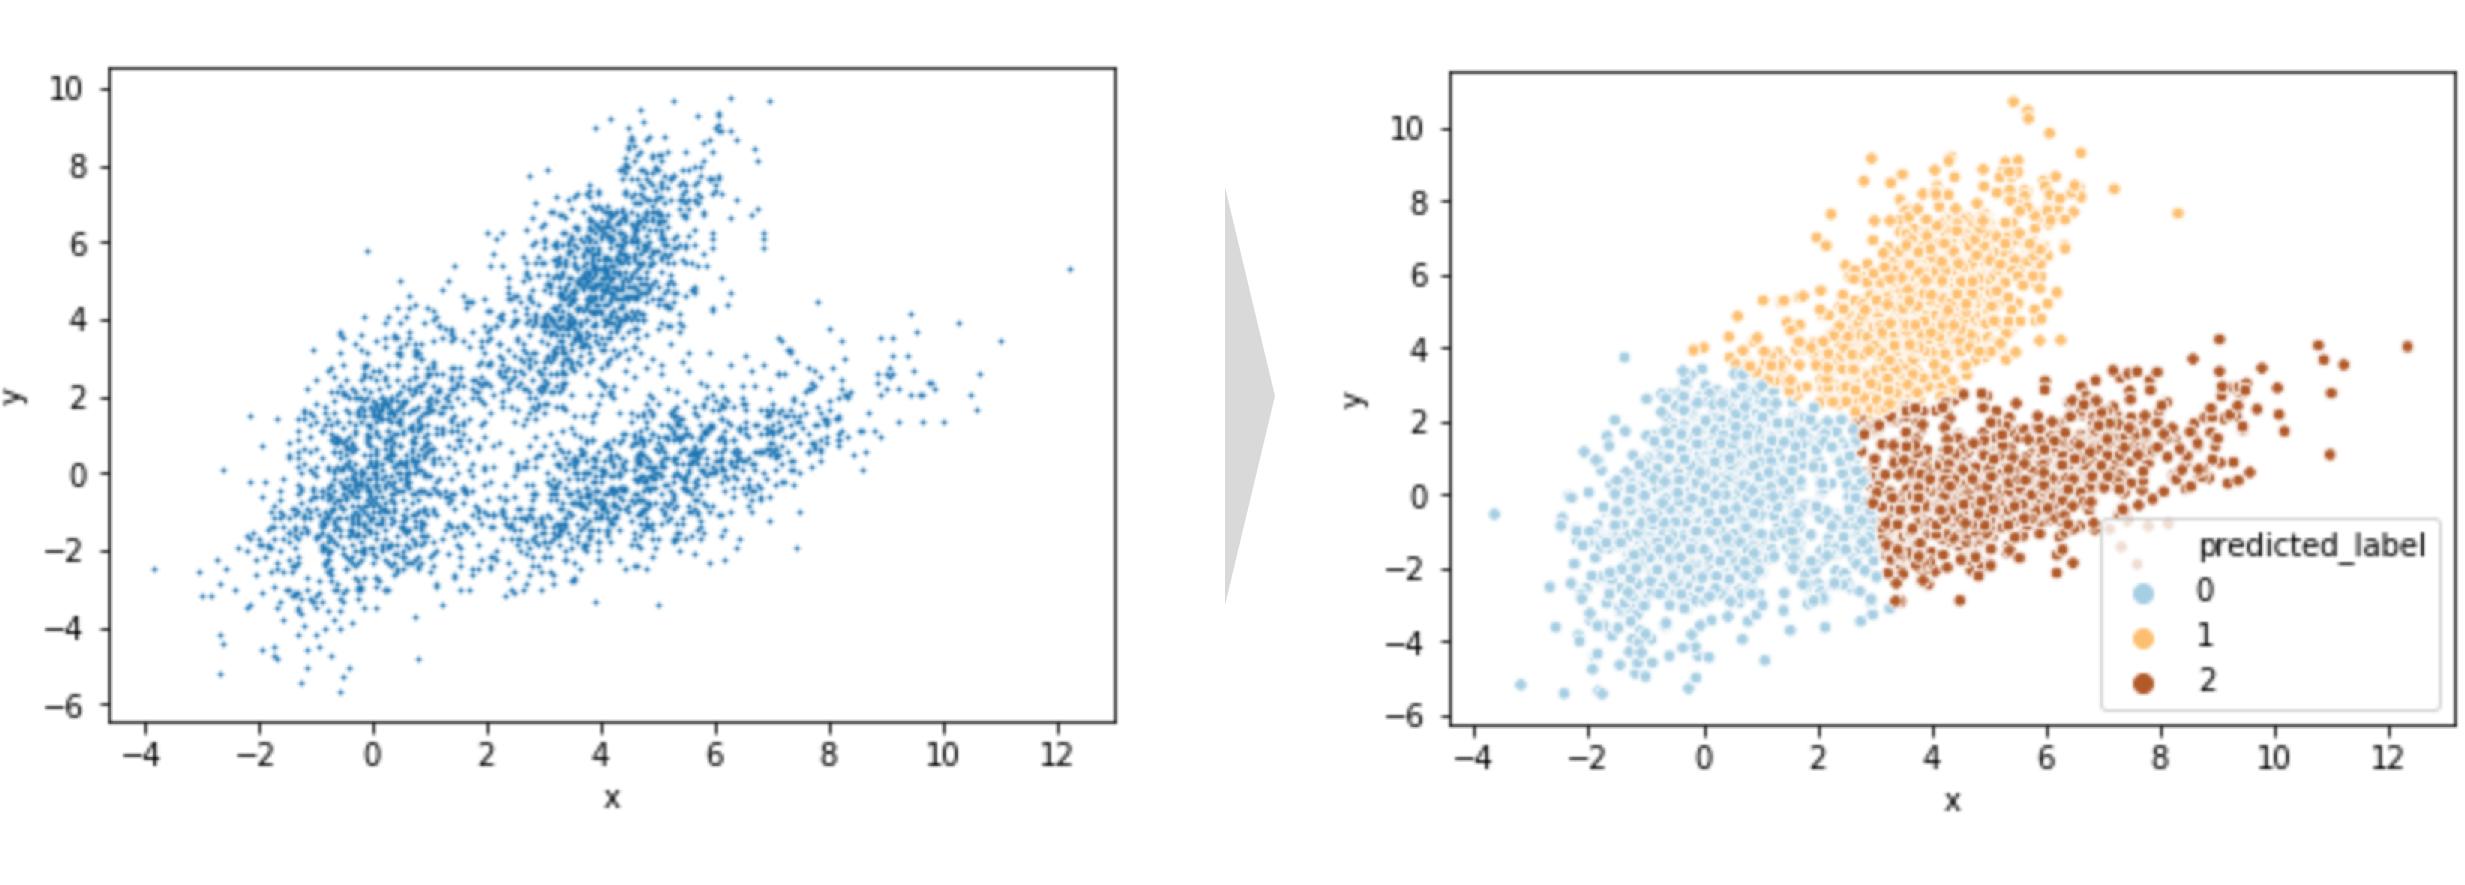
\includegraphics[width=0.7\linewidth]{../img/clystyrau_k_modd}
\caption{Cyn ac ar \^{o}l clystyru k modd.}
\end{center}
\end{figure}
I rhoi enghraifft i'r llun uchod, dychmygwch fod un echelin yn cynrychioli rhif myfyrwyr ag yr llall yn cynrychioli marc cyfartaledd yn mhob pwnc. Efallai fod eisiau rhannu y myfyrwyr i 3 dosbarth(k). Fysa clystyru k-modd medru dosrannu y myfyrwyr gan edrych ar phob pwnc yn unigol i wneud yn siwr fod y myfyrwyr tebyg yn cael ei rhoi gyda'i gilydd. Mi wnawn edrych y nawr ar yr set data iris sy'n boblogaidd iawn yn y maes ystadegaeth a gwyddor data. Mae'r data yn cynnwys mesuriadau uchder ag lled petal a setal 150 planhigyn iris. Yn isod gweler lun o allbwn clystyru k-modd yn erbyn y clystyrau gwreiddiol o'r data. Gwelwyd fod yr algorithm yn neud yn wych! 
\begin{figure}[h!]
\begin{center}
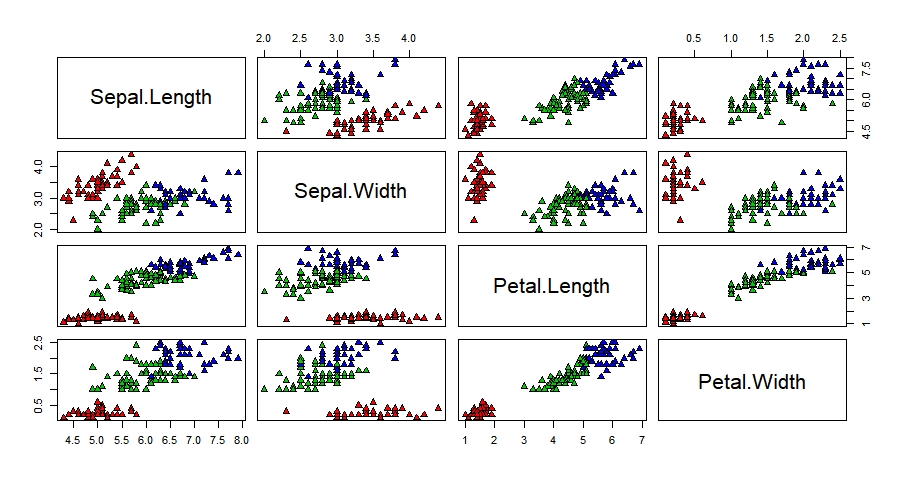
\includegraphics[width=0.5\textwidth]{../img/enghraifftclystyru.jpeg}
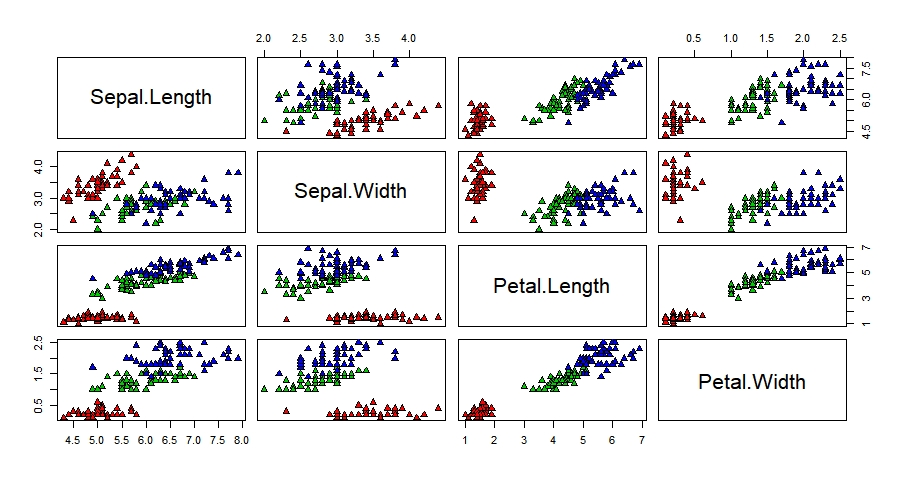
\includegraphics[width=0.5\textwidth]{../img/Actualclassification.jpeg}
\caption{Clystyrau k-modd yn erbyn y clystyrau gwreiddiol o'r data wedi'i labelu}
\end{center}
\end{figure}
\section{Sut mae Clystyru K-modd yn gweithio?}
\section{Tiwtorial yn R}
Yn y tiwtorial hyn, mi wnawn cerdded drwodd y dull i creu y clystyrau a wnaethom gweld gynnar ar y set data iris.
\begin{enumerate}
	\item Y Pecynnau \\
Fydd angen lawrlwytho a gosod y pecynnau "graphics", "stats" ag "datasets" ar eich fersiwn chi o R studio. Ffordd hawdd i gwirio hyn fydd i ddefnyddio y ffwythiant library("enw'r pecyn") ac os fydd yna gwall yna defnyddiwch y ffwythiant install.packages("enw'r pecyn")
	\item Y C\^{o}d \\
Mae'r data iris ar gael iddym drwy'r pecyn "datasets". Yn yr enghraifft top mi wnaethom defnyddio k fel 3, felly hyna be wnawn neud eto.
Dyma'r c\^{o}d ar gyfer rhedeg clystyru k-modd:
\begin{minted}{r}
clysteru_tri <- kmeans(iris[,1:4],3, nstart = 20)
clysteru_tri 
\end{minted}
Mae'r llinell gyntaf o c\^{o}d yn rhedeg clystyru k-modd ar y set data iris gyda k=3. Mae'r darn nstart yn cynrychioli faint o dosraniadau i drio yn cychwyn yn erbyn'r ffwythiant amcan, er mwyn dewis y cychwyn orau. Mae'r ail linell yn allbwn yr wybodaeth canlynol:
\begin{minted}{r}
>>>K-means clustering with 3 clusters of sizes 50, 62, 38
>>>
>>>Cluster means:
>>>  Sepal.Length Sepal.Width Petal.Length
>>>1     5.006000    3.428000     1.462000
>>>2     5.901613    2.748387     4.393548
>>>3     6.850000    3.073684     5.742105
>>>  Petal.Width
>>>1    0.246000
>>>2    1.433871
>>>3    2.071053
>>>
>>>Clustering vector:
>>>  [1] 1 1 1 1 1 1 1 1 1 1 1 1 1 1 1 1 1 1 1 1 1 1
>>> [23] 1 1 1 1 1 1 1 1 1 1 1 1 1 1 1 1 1 1 1 1 1 1
>>> [45] 1 1 1 1 1 1 2 2 3 2 2 2 2 2 2 2 2 2 2 2 2 2
>>> [67] 2 2 2 2 2 2 2 2 2 2 2 3 2 2 2 2 2 2 2 2 2 2
>>> [89] 2 2 2 2 2 2 2 2 2 2 2 2 3 2 3 3 3 3 2 3 3 3
>>>[111] 3 3 3 2 2 3 3 3 3 2 3 2 3 2 3 3 2 2 3 3 3 3
>>>[133] 3 2 3 3 3 3 2 3 3 3 2 3 3 3 2 3 3 2
>>>
>>>Within cluster sum of squares by cluster:
>>>[1] 15.15100 39.82097 23.87947
>>> (between_SS / total_SS =  88.4 %)
\end{minted}
Mae'r c\^{o}d uchod rhoi pob wybodaeth a fysa chi eisiau wybod fel allbwn o'r proses.
I weld y clysterau allwn plotio graff ar gyfer phob cyfuniad o newidynnau. Mae hyn yn alluogi ni i weld yr gwaith dpsbarthu mae'r algorithm wedi'i neud.
\begin{minted}{r}
plot(iris[,1:4], pch = 24, bg=c("red","green3","blue")[unclass(clysteru_tri$cluster)])
\end{minted}
Yn y ffwythiant "plot" uchod, mae'r darn gynta ohono yn cyfeirio tuag at pa data fydd yn cael ei clysteru. Mae'r ail darn yn penodi be fydd pob pwynt data yn cael ei cynrychioli fel pan mae'r darn dwythaf yn penodi lliw i pob clwstwr.
\end{enumerate}
